
\subsubsection{Artefact granularity}\label{sec:granularity}

Project stakeholders must decide on the appropriate level of trace granularity for each artifact type. For example, when tracing to UML class diagrams, they could generate a trace at the package, class, or method level.
Granularity must be carefully determined to effectively support stakeholders in their traceability tasks, while minimizing the effort involved to analyze and utilize the set of returned trace links. This can be especially problematic
in large, weakly structured documents that might not contain clearly defined components at the desired granularity level. To mitigate this problem, automated traceability tools can cluster sentences into meaningful semantically related groups and then generate traces to those groups~\cite{clelandhuang2007bestPracticeForAutomatedTraceability}.

As can be seen in Figure \ref{fig:mm-granularity}, We distinguish between five main types of artefacts: i) natural language and unstructured text documents are \texttt{TextArtefacts}, ii) executable test unit and suites are \texttt{TestArtefacts}, iii) models at design or conceptual level are \texttt{ModelArtefacts}, and iv) source code document, SQL sources, scripts and configuration documents are \texttt{CodeArtefacts}. They are all specialization of Artefact. Types differ in the nature of the structure of the artefacts. This is an arbitrary separation grounded on our experience with traceability. Other can be easily introduced to span closer to user needs.
An \texttt{ArtefactFragment} is a part of an Artefact. It can be subdivided into sub-fragments.
\begin{figure}[ht]
	\centering
	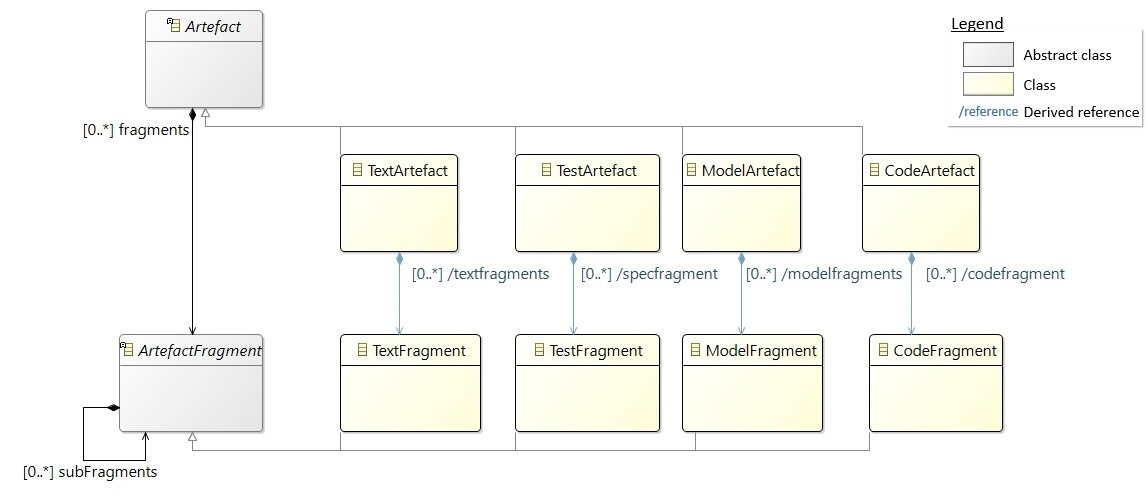
\includegraphics[width=.99\linewidth]{images/granularity.jpg}
	\caption{Customizable granularity}
	\label{fig:mm-granularity}
\end{figure}

Note that we could also opt for a rather simpler approach where artefact types are not modeled as subclasses but where we would just have a single attribute \texttt{ArtefactType} in \texttt{Artefact}. The obvious disadvantage with this option is that we lose the opportunity to add information relevant only to specific types of artefacts.

\paragraph{Classes}
\begin{itemize}
    \item A \texttt{TextArtefact} is a(n) (un)structured text document. \texttt{TextArtefacts} can further decompose into \textit{Sections}, \textit{Subsections}, and \textit{Paragraph}. Each of them may contain \textit{part-Of-Speech} that points to concepts in the application domain.
    
    \item A \texttt{ModelArtefact} is an artefacts related to a model-level representation. \texttt{ModelArtefacts} can be UML, SysML or other types of models, with a structural hierarchy inherent to their entity-relation form. In the case of UML, a decomposition may follow the \textit{Package}, \textit{Class}, \textit{Methods}, \textit{Attributes}, and \textit{References} hierarchical scheme. \textit{Named Elements} point to unique elements of the language uniquely identified.
    
    \item A \texttt{CodeArtefact} is a documents containing source code independently of the specific programming language. \texttt{CodeArtefacts} may decompose into \textit{CodeBlock}, \textit{Header}, \textit{Variable}, \textit{Methods}, and so on. 
    
    \item A \texttt{TestArtefact} is a test unit or suite.
    
    \item And so forth and so on for their respective fragments.
    
\end{itemize}

\pagebreak
\paragraph{Well-formedness rules}
Well-formedness rules are expressed as OCL constraints. 
Rules in Figure \ref{fig:ocl-granularity} the coherence between subtypes of artefacts, fragments, and subfragments. 
\begin{figure*}[h]
\centering 
\rule{0.9\linewidth}{1pt}
\vspace{-0.2truecm}
\small
\begin{ocl}[0.85\linewidth]

\vspace{0.3truecm}\OCLcontext~TextArtefact \OCLinv ~textFragmentsTyping: 
\\ \verb+     + \OCLself.fragments \OCLarrow forAll(\OCLself \OCLarrow oclIsKindOf(TextFragment)

\vspace{0.3truecm}\OCLcontext~CodeArtefact \OCLinv ~codeFragmentsTyping: 
\\ \verb+     + \OCLself.fragments \OCLarrow forAll(\OCLself \OCLarrow oclIsKindOf(CodeFragment)

\vspace{0.3truecm}\OCLcontext~ModelArtefact \OCLinv ~modelFragmentsTyping: 
\\ \verb+     + \OCLself.fragments \OCLarrow forAll(\OCLself \OCLarrow oclIsKindOf(ModelFragment)

\vspace{0.3truecm}\OCLcontext~TestArtefact \OCLinv ~testFragmentsTyping: 
\\ \verb+     +\OCLself.fragments \OCLarrow forAll(\OCLself \OCLarrow oclIsKindOf(TestFragment)


\vspace{0.3truecm}\OCLcontext~TextFragment \OCLinv ~textsubfragmentsTyping: 
\\ \verb+     + \OCLself.subfragments \OCLarrow forAll(\OCLself \OCLarrow oclIsKindOf(TextFragment)

\vspace{0.3truecm}\OCLcontext~CodeFragment \OCLinv ~codesubfragmentsTyping: 
\\ \verb+     + \OCLself.subfragments \OCLarrow forAll(\OCLself \OCLarrow oclIsKindOf(CodeFragment)

\vspace{0.3truecm}\OCLcontext~ModelFragment \OCLinv ~modelsubfragmentsTyping: 
\\ \verb+     + \OCLself.subfragments \OCLarrow forAll(\OCLself \OCLarrow oclIsKindOf(ModelFragment)

\vspace{0.3truecm}\OCLcontext~TestFragment \OCLinv ~testsubfragmentsTyping: 
\\ \verb+     +\OCLself.subfragments \OCLarrow forAll(\OCLself \OCLarrow oclIsKindOf(TestFragment)


\vspace{0.3truecm}\OCLcontext~NamedElement \OCLinv ~noNestedNamedElements: 
\\ \verb+     +\OCLself.namedelementsDefined \OCLarrow isEmpty()  \OCLand
\\ \verb+     +\OCLself.namedelementsUsed \OCLarrow isEmpty() \OCLand
\\ \verb+     +\OCLself.subfragments \OCLarrow isEmpty() 
\end{ocl}

\vspace{0.4truecm}
\rule{0.9\linewidth}{1pt}
\vspace{-0.2truecm}

\caption{OCL constraints over elements of the granularity package.}
\label{fig:ocl-granularity}
\vspace{-0.6truecm}
\end{figure*}


\paragraph{Illustrative example}%Granularity

A trace starts with the PoSs we want to trace down to the design level. It also contains the successive containment connections from document, to section, to PoS in order to refine the granularity of the results to sections instead of whole documents. The trace also contains the link between PoSs and their corresponding model entities, as well as model entities hierarchy (\textit{e.g.,} the class, method, or package they belong to).

To summarize:
\begin{itemize}
    \item A text \texttt{Document} is a \texttt{TextArtefact}. It is decomposed into \texttt{Sections}. Sections define or use \texttt{PoSs}. Both Sections and PoSs are \texttt{TextFragment} (derived from \texttt{ArtefactFragment}).
    \item A Papyrus \texttt{Model} is a \texttt{ModelArtefact}. It is decomposed into modelling elements : \textit{e.g.,} \texttt{Packages}, \texttt{Classes}, and \texttt{Structural features}. They are \texttt{ModelFragments}. \texttt{ModelFragments} (spceializations of \texttt{ArtefactFragments}) define and use \texttt{NamedElements} (\textit{i.e.,} elements of the system with unique identifier). 
\end{itemize}
\begin{figure}[ht]
	\centering
	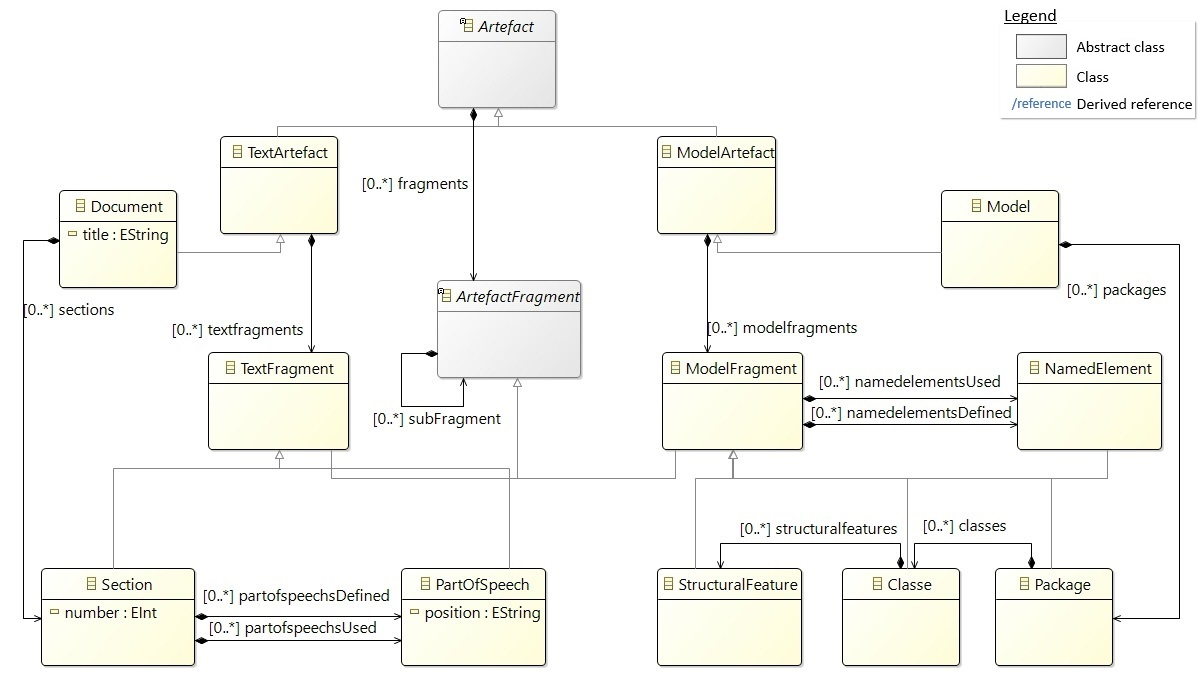
\includegraphics[width=.99\linewidth]{images/granularity-re.jpg}
	\caption{Granularity customized for certification to model transclusion}
	\label{fig:mm-granularity-re}
\end{figure}
